\section{Les classes \enquote{agents}}
Lors du premier sprint, nous avons dû mettre en place la base du programme. Nous avions prévu de faire l'UML~\ref{v0.1} page~\pageref{v0.1}.

 Pour le modèle, il s'agissait de mettre en place les classes :
\begin{itemize}
\item Turtle qui représente une tortue, 
\item Point, pour stocker les coordonnées d'une tortue,
\item Line, qui est composé de points, et qui permet aux tortues de laisser une trace (instruction pendown),
\item World.
\end{itemize}


\begin{figure}[h]
\caption{\label{v0.1} UML de la version 0.1 prévue}
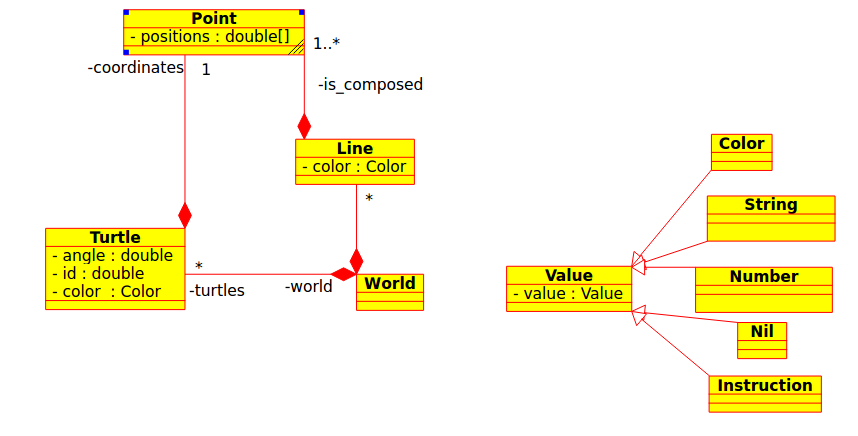
\includegraphics[scale=0.5]{doc/report/uml/v01.png}
\end{figure}


La classe World représente le monde des tortues. Il contient la liste des tortues, et les lignes tracées par ces tortues.
A la fin du sprint 1, on pouvait voir une tortue avancer et tracer une ligne sur sur passage.
Nous avions réalisé le schéma~\ref{v0.1R} page~\pageref{v0.1R}, en dehors de la classe Instruction.


Pour le second sprint, nous avons ajouté une classe Agent, car les classes World, Turtle et Zone sont des agents, au sens multi-agent (cf ~\ref{v0.2} page~\pageref{v0.2}) . Elle contient le code en commun de ces trois classes.
 
Ils ont chacun un parent, celui qui l'a créer, une liste d'enfants, et des propriétés. Les propriétés sont des variables définit par l'utilisateur lors de la définition du code de l'agent, donc surtout utile pour les tortues.


Le monde a une taille, une liste de \enquote{breed}, d'espèce. Il y a les espèces nommées et les \enquote{anonymes}, qui sont des turtles dans le code.


Comme le montre ce code, on peut créer des tortues nommées ou pas. Une tortue anonyme s'écrit \enquote{new agent} et une nommée \enquote{agent listener}.\\


\begin{lstlisting}
agent listener () {
	fd 2
}

new listener ()

new agent {
	lt 30
	fd 5
}
\end{lstlisting}
Lors du troisième sprint, nous avons mis en place des pointers intelligents dans toutes nos classes.


Le but de ce sprint était la mise en place de la communication entre les agents. Les tortues peuvent communiquer avec les zones par écriture dans leurs propriétés. Les tortues peuvent communiquer entre elles grâce à des méthodes comme sendAll(message), recv(), etc 
(cf figure~\ref{v0.3} page~\pageref{v0.3}).


Ensuite, nous devions ajouter des fonctionnalités tel que la maîtrise du temps et l'exportation du modèle. Ces ajouts ne provoquent pas de changement du coté du modèle, si ce n'est quelques méthodes dans les classes World et Turtle et Zone pour l'exportation du modèle.


L'exportation du modèle consiste à créer une sauvegarde de l'état du modèle à un instant t dans un fichier JSON.


Cela permettra ensuite, en passant par une transformation en CSV, d'avoir un tableau avec toutes ces données, ce qui offre la possibilité d'avoir des diagrammes de l'évolution du monde.



La maîtrise du temps se fait grâce à un bouton pause, qui arrête les threads qui s'exécutent, ou par un slider qui permet de ralentir ou de diminuer la vitesse. Cela se fait dans le code grâce à une méthode sleepfor() qui prend en paramètre un temps donné.


\section{Les types}
Lors du premier sprint, nous mettions en place certains types Stibbons, comme Color, pour la couleur, ou Nil qui a une valeur nulle. Ils héritent de Value, une classe abstraite qui contient une valeur et ses accesseurs.


Les instructions tel que pendown, forward, etc, sont finalement des mots clés dans la grammaire du langage, et non pas des instructions, contrairement à ce que nous avions prévu (UML~\ref{v0.1} correspondant page~\pageref{v0.1}).\\


\begin{figure}[h]
\caption{\label{v0.1R} UML de la version 0.1 réalisée}
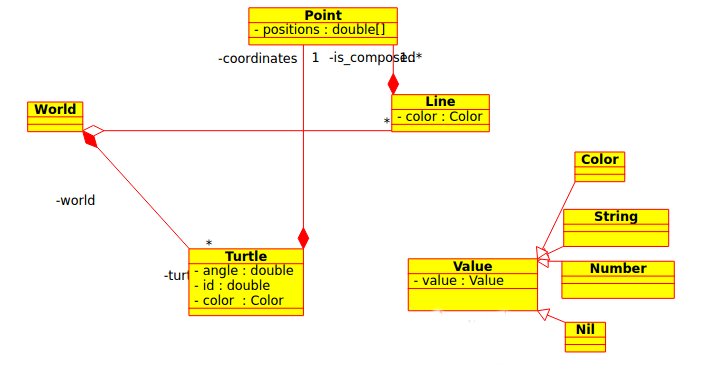
\includegraphics[scale=0.5]{doc/report/uml/v01reel.png}
\end{figure}

Lors du sprint deux, les types stibbons sont les mêmes, mais leurs définitions s'est un peu compléxifiées en passant par une classe Simple-value, pour la mise en place des mutexs. Une énumeration des types Stibbons existe, elle est utiliser avec la méthode getType() pour pouvoir connaître le type de Value.


Pour que l'utilisateur puisse écrire des fonctions dans le code, nous avons ajouté une classe Function, qui stocke un arbre, qui contient le code la fonction, déjà parsé.
\\ Des mutexs ont été ajouté dans toutes les classes pour assurer que les threads sont thread-safe (cf figure~\ref{v0.2} page~\pageref{v0.2}).


A la fin de ce sprint, nous devions relancer le programme pour charger un nouveau fichier de code, ce qui n'était pas pratique.



\begin{figure}[h]
\caption{\label{v0.2} UML version 0.2}
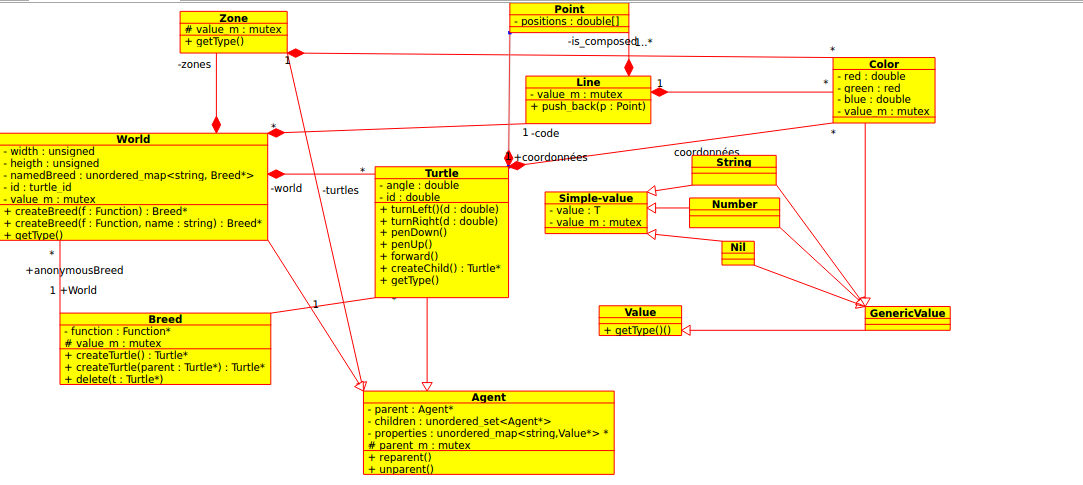
\includegraphics[scale=0.45]{doc/report/uml/v02.png}
\end{figure}

Lors du troisième sprint, nous avons ajouté des sous-classes de Function Standart-function et User-function pour représenter les fonctions standarts du langages (cf figure~\ref{v0.3} page~\pageref{v0.3}) .
\begin{figure}[h]
\caption{\label{v0.3} UML version 0.3}
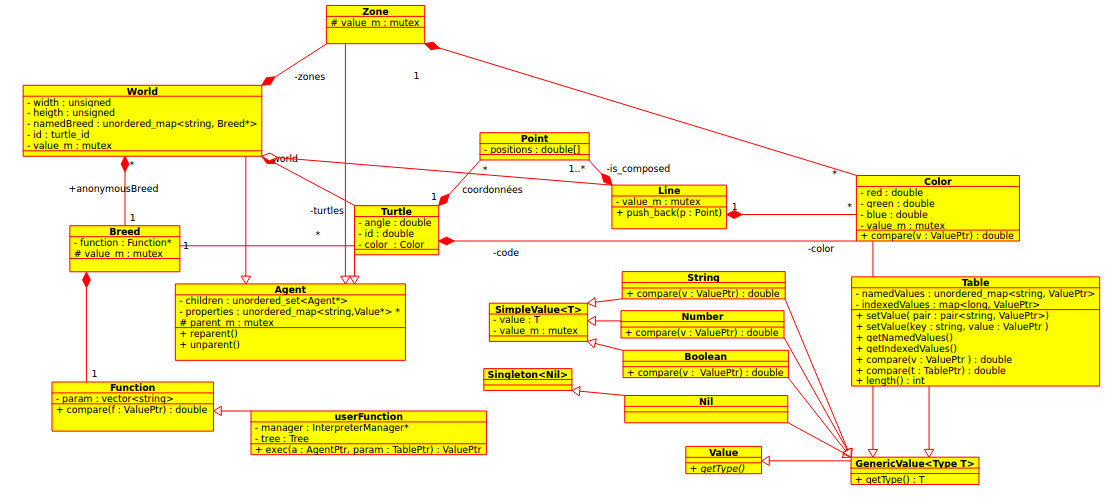
\includegraphics[scale=0.4]{doc/report/uml/v03.png}
\end{figure}
On les différencie des instructions par leurs parenthéses derrière leur nom.\\ Les User-function représentent les fonctions crées par l'utilisateur.\\
L'ajout de table fait aussi partit de ce sprint. Nous avons choisi, pour notre langage un seul type de conteneur : les tableaux.
Nous avons choisi de les écrire façon php, avec des accolades.\\
\begin{lstlisting}
a = 12

t = {18,red,"bla"}
v = { "bla" : "blou", "blue" : blue, a : 29 }

println(t[2])
t[2] = 32
println(t[2])
v[] = 48
println(v)

u = 5 new agent {
	while true fd 20
}
\end{lstlisting}
Le sprint 5 n'apporte pas de grand changement dans le modèle. Notre UML définitif est donc celui du sprint 4.

